Como ya se ha indicado, el proyecto llevaría 7 meses de desarrollo. La inversión inicial ascendería a un total de, 81429.16 €, cabe recordar, que durante el tiempo de producción también hay gastos debido al mantenimiento del proyecto y que se tardará, aproximadamente, 22 meses en recuperar la inversión inicial más el dinero invertido en el mantenimiento. Además, no se han tenido en cuenta gastos en alquiler de una oficina, mantenimiento de esta ni gastos en contratiempos como reparación de los equipos de la oficina, etcétera. 

Al igual que en la mayoría de proyectos de desarrollo de software, el mayor gasto se ha ido en mano de obra. En la siguiente tabla se reflejan las horas de trabajo que supone cada tarea y el coste en €/h de cada una.
\\
\begin{ThreePartTable}
\label{table:tareas}
\captionof{table}{Gastos derivados de la mano de obra utilizada durante el desarrollo}
\begin{tabularx}{0.9\textwidth} { 
  | >{\raggedright\arraybackslash}X
  | >{\raggedright\arraybackslash}X
  | >{\raggedleft\arraybackslash}X | }
    \hline \textbf{Tareas} & \textbf{Horas de trabajo} & \textbf{Costo}\\
    \hline Análisis & 416 & 3696 €\\
    \hline Diseño & 104 & 3535,68 €\\
    \hline Desarrollo & 1224 & 39203,36 €\\
    \hline Despliegue & 320 & 10324 €\\
    \hline Control proyecto & 116,40 & 4656 €\\
    \hline Total & 2180,40 & 69815,04 €\\
    \hline 
\end{tabularx}
\end{ThreePartTable}

En el siguiente diagrama se muestra la distribución del dinero invertido en mano de obra durante el desarrollo.

\begin{figure}[H]
    \centering
    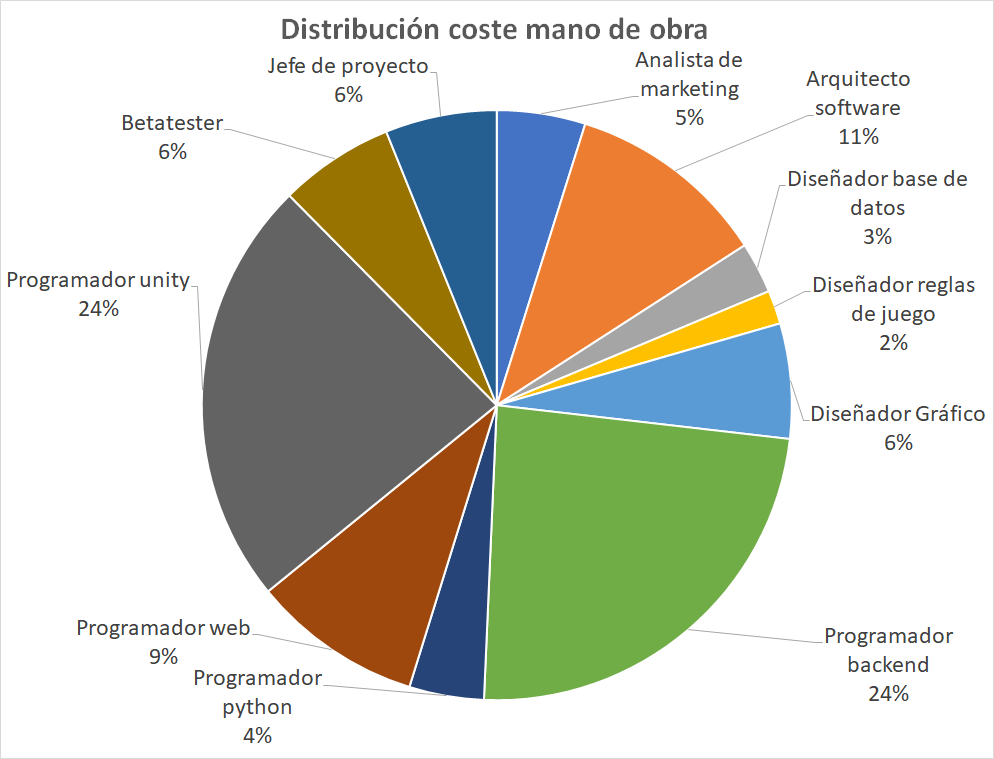
\includegraphics[width=1\textwidth]{Memoria_TFG_LaTeX/images/distribucionGastosManoDeObra.PNG}
    \caption{Distribución de los gastos de la mano de obra durante el desarrollo del proyecto.}
    \label{fig:distribucionGastosManoDeObra}
\end{figure}

El otro gasto que ocurre durante el desarrollo son los gastos en material, en este caso, se tratan de los equipos informáticos de los empleados.

\begin{ThreePartTable}
\label{table:material}
\captionof{table}{Gastos derivados de la compra de hardware durante el desarrollo}

\begin{tabularx}{0.9\textwidth} { 
  | >{\raggedright\arraybackslash}X
  | >{\raggedright\arraybackslash}X
  | >{\raggedright\arraybackslash}X
  | >{\raggedleft\arraybackslash}X | }
    \hline \textbf{Material} & \textbf{Unidades} & \textbf{Costo unidad} & \textbf{Costo}\\
    \hline Teclado & 3 & 11 € & 33 €\\
    \hline Ratón & 3 & 18 € & 54 €\\
    \hline Ordenador Sobremesa & 3 & 860 € & 2580 €\\
    \hline Ordenador Portátil & 1 & 591 € & 591 €\\
    \hline Pantalla & 3 & 195 € & 585 €\\
    \hline Móvil Android & 1 & 215 € & 215 €\\
    \hline Móvil iOS & 1 & 206 € & 206 €\\
    \hline \textbf{Total} &  &  & \textbf{4264 €}\\
    \hline
\end{tabularx}

\end{ThreePartTable}


Como se mencionó anteriormente, la mayor parte del coste de desarrollo se ha invertido en mano de obra. En el siguiente gráfico se puede observar la gran diferencia entre el gasto de mano de obra y el gasto en material.
\begin{figure}[H]
    \centering
    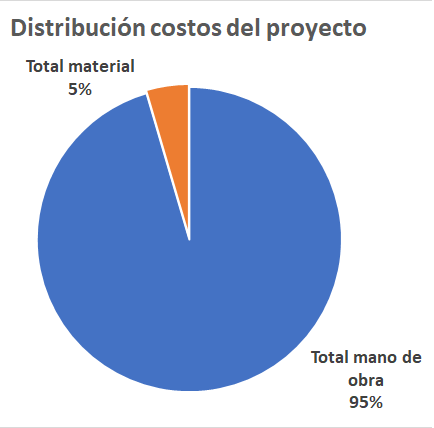
\includegraphics[width=0.75\textwidth]{Memoria_TFG_LaTeX/images/distribucionGastosDesarrollo.PNG}
    \caption{Distribución de los gastos durante el desarrollo del proyecto.}
    \label{fig:distribucionGastosDesarrollo}
\end{figure}